\chapter{Prototype Design}
\label{chap:prototype}

\section{Overview}

Throughout the course of this dissertation work, the Rapidly Reconfigurable Research Cockpit (R3C) prototype underwent many changes and improvements to the technology used.
Our underlying motivation and goals of the technical approach of the prototype remained constant, but as technology evolved and our experience and feedback grew, a number of improvements and revisions were developed.
In this chapter, three major versions of the prototype are outlined, and the evolution of the technical approach is described.
The first prototype was not used in a formal experiment, but two versions based on the second prototype were used for the first two research studies (Chapters~\ref{chap:pointing}~and~\ref{chap:ph_exp}).
The final prototype was used in the third experiment (Chapter~\ref{chap:de_exp}).

\section{Requirements}

The following high level requirements for the Rapidly Reconfigurable Research Cockpit (R3C) prototype originated from the motivation described in Section \ref{sec:intro_overview}.
These requirements guided the development of the prototypes, based on the technology available.

\begin{description}
    \item [Rapid prototyping of physical mockup.]
        Based on the motivation of enabling more rapid redesign iterations, the R3C system should allow for rapid changes in the physical representation of the cockpit (the mockup) without needing to undertake large software or hardware reconfigurations.
    \item [Immersive head-mounted display.]
        The need for an immersive HMD with a large field of view is based on the need to use the system as a design evaluation tool.
        Without the ability to place visuals on the screens or create out-the-window views, design evaluations may not be as useful.
        Current augmented reality or mixed reality goggles do not provide the same level of immersion that a fully-virtual HMD provides.
    \item [Unobtrusive hand tracking.]
        For a realistic design evaluation, it is important that the hand tracker does not modify the users behavior or inhibit their tactile sense.
        Many hand trackers use a glove or other marker worn on the hand to provide the tracking ability.
        Wearing a glove to achieve hand tracking would remove one of the benefits of the R3C system -- providing a realistic tactile sensory input.
        Newer optical-based hand trackers allow this requirement to be fulfilled.
    \item [Minimal setup and calibration.]
        Our goal is to provide a system that can be used ``on top'' of existing mockup systems without extensive modifications.
        One consequence of this means that as much as possible, the hardware used must be easy to set up and able to use in constrained spaces.
        This requirement eliminates some of the high-end head-mounted displays that use complicated head tracker systems requiring precise calibration.
        Our solution also proposes the use of hand tracking to recognize the pilots' input without the need for outfitting the mockup with working input actuators (i.e.\ buttons).
        Past approaches to hand tracking which use multiple precisely calibrated cameras, or magnetic sensors in a well-defined magnetic field, will not satisfy this requirement.
\end{description}

\section{Prototype Development}

\subsection{First Prototype}

The first prototype was a proof of concept system, providing a platform for the future prototypes.
The major components of the first prototype were:
\begin{itemize}
    \item Oculus Rift Development Kit (VR HMD)
    \item LeapMotion (hand tracker)
    \item 3D Printed Cockpit Instrument
    \item EDGE Rendering Engine with custom software for integration
\end{itemize}

This prototype was quickly outdated with new technology and software updates before it could be used for a formal research study.
However, many informal feedback sessions did help highlight the usability and technical issues that led to the next prototype.
The software developed during this prototype also provided a significant base for the software used throughout all the prototypes.
The hardware used for this prototype was the first generation Oculus Rift Development Kit and the first generation of software for the LeapMotion hand tracker.

\subsubsection{Rendering Engine}

We are using a NASA developed rendering engine named EDGE to provide the visuals for the virtual scene rendered in the head-mounted display (HMD).
EDGE is highly customizable and extendable through C/C++ plugins, Tcl scripts, or networking functions.
Many of the integrations described in the prototypes were created as EDGE plugins.
This rendering engine was used in all subsequent prototypes and research studies.

\subsubsection{Virtual Reality Headset}

The head-mounted display (HMD) we used for the first prototype was an Oculus Rift Development Kit (Figure~\ref{fig:proto_oculus}).
The lightweight headset provides an immersive virtual reality experience by combining a wide field-of-view scene with accurate head tracking, giving a stable virtual world.
The small display (cell phone sized) is viewed through a single set of lenses.
A unique image is presented to each eye, providing stereoscopic 3D vision.
The orientation of the head is tracked using internal sensors (accelerometer, gyroscope and magnetometer) and exposed through the software developer’s kit (SDK).
%The and this was developed into an EDGE plugin.
The first generation Oculus Rift Development Kit has a 1280x800 LCD screen (with 640x800 for each eye) with a refresh rate of \SI{60}{\hertz}.
The field of view is approximately \ang{110}.

\begin{figure}
    \centering
    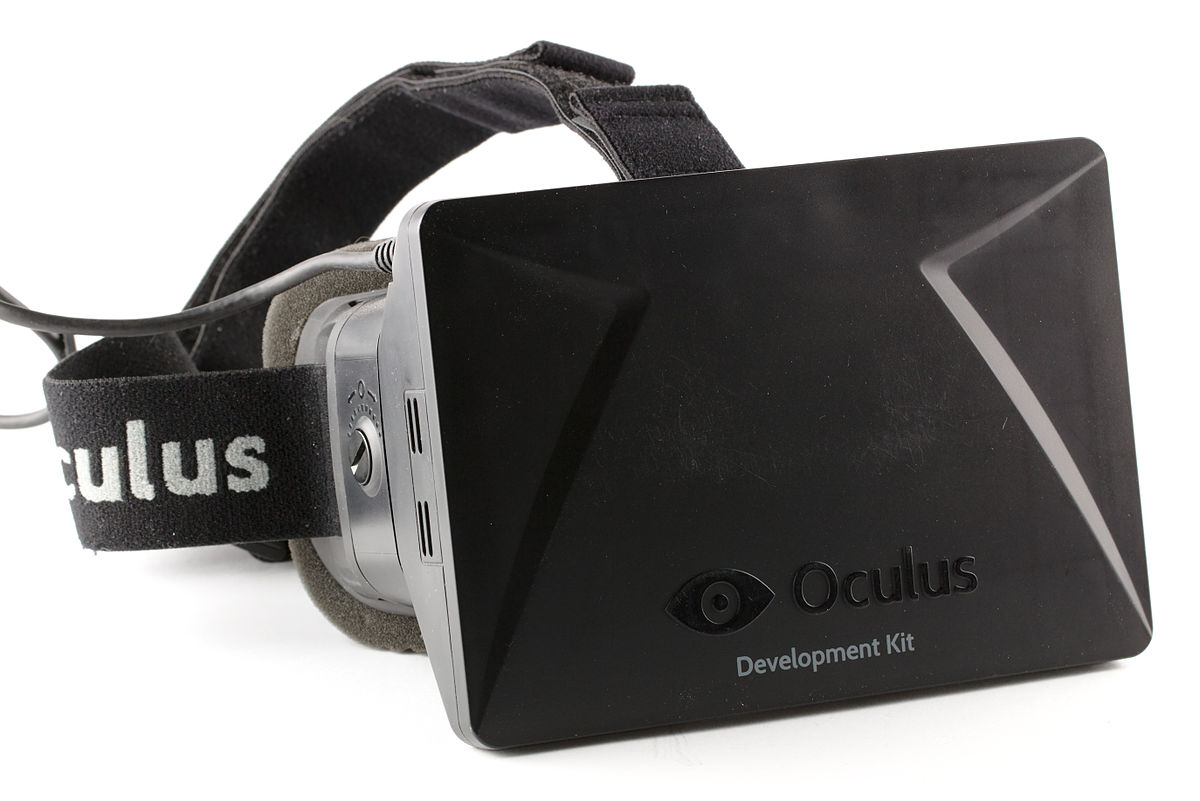
\includegraphics[width=3in]{proto_dk1.jpg}
    \caption{The original Oculus Rift Development Kit.}
    \label{fig:proto_oculus}
\end{figure}

\subsubsection{3D Printed Instruments}

A central tenant of our technical approach is to use physical, geometrically accurate instrument shapes that provide tactile feedback to the fingertips, but no functionality (i.e.\ no screens, no working buttons, etc.).
In order to achieve this, we have produced 3D printed ``instruments'' that can be easily rearranged on a panel mount (pegboard).
An instrument in a cockpit can be defined as any device that provides information about or provides control of the airplane and its flight situation.
In our case, the instruments we prototype consist of a device with buttons and screens in a variety of geometrical configurations and layouts.
Since the devices are rapidly prototyped, they can be redesigned much more rapidly than functioning simulator instruments.
By placing the geometrically accurate 3D printed instruments at the correct cockpit locations, the user is provided with accurate tactile feedback without the need for stimulating true touch with virtual haptic feedback.

To use an instrument in the R3C system, it requires two versions of the 3D model.
The first is the version for the rendering engine, which requires textures and possible work to reduce the number of polygons so that rendering is not slowed down by model complexity.
The second model is for the 3D printing, which depending on the 3D printer used, will often require small changes to allow for a successful print.
Both of these formats require a surface mesh model.
Often, the original version exists as a CAD (Computer-Aided Design) model which typically does not describe the surface mesh directly but instead describes the geometric models that define the part.
The difficulty of the conversion from CAD to a surface mesh depends on the model and the requirements of the rendering engine.

For this initial prototype, a demonstration instrument was developed based on a large multi-function display with edge keys.
This design was chosen based on their standard use in current aircraft and spacecraft cockpits (e.g.\ see \citet{us_department_of_defense_department_1999}) and was based off the current design for the NASA Orion spacecraft cockpit (Figure~\ref{fig:orion_sim}).
The instrument model as viewed in the rendering engine is shown in Figure~\ref{fig:proto_mfd_render}.
The 3D printed version is shown pictured in Figure~\ref{fig:proto_mfd_print}.
Since it is only used for the tactile feel, it has a plain aesthetic.
The color and visual detail of the instrument are only on the rendered model in the virtual world, simplifying the physical prototyping process.
This instrument was also 3D printed in segments due to the limitations of the printer used, but this did not affect the virtual representation.
Figure~\ref{fig:proto_first_panel} shows the instrument mounted on a panel and being used.
This instrument provided a base for the demos.
Although this specific design was not used in a research study, the workflow learned to create this demo instrument was used for future instruments utilized in the research studies.

\begin{figure}
    \centering
    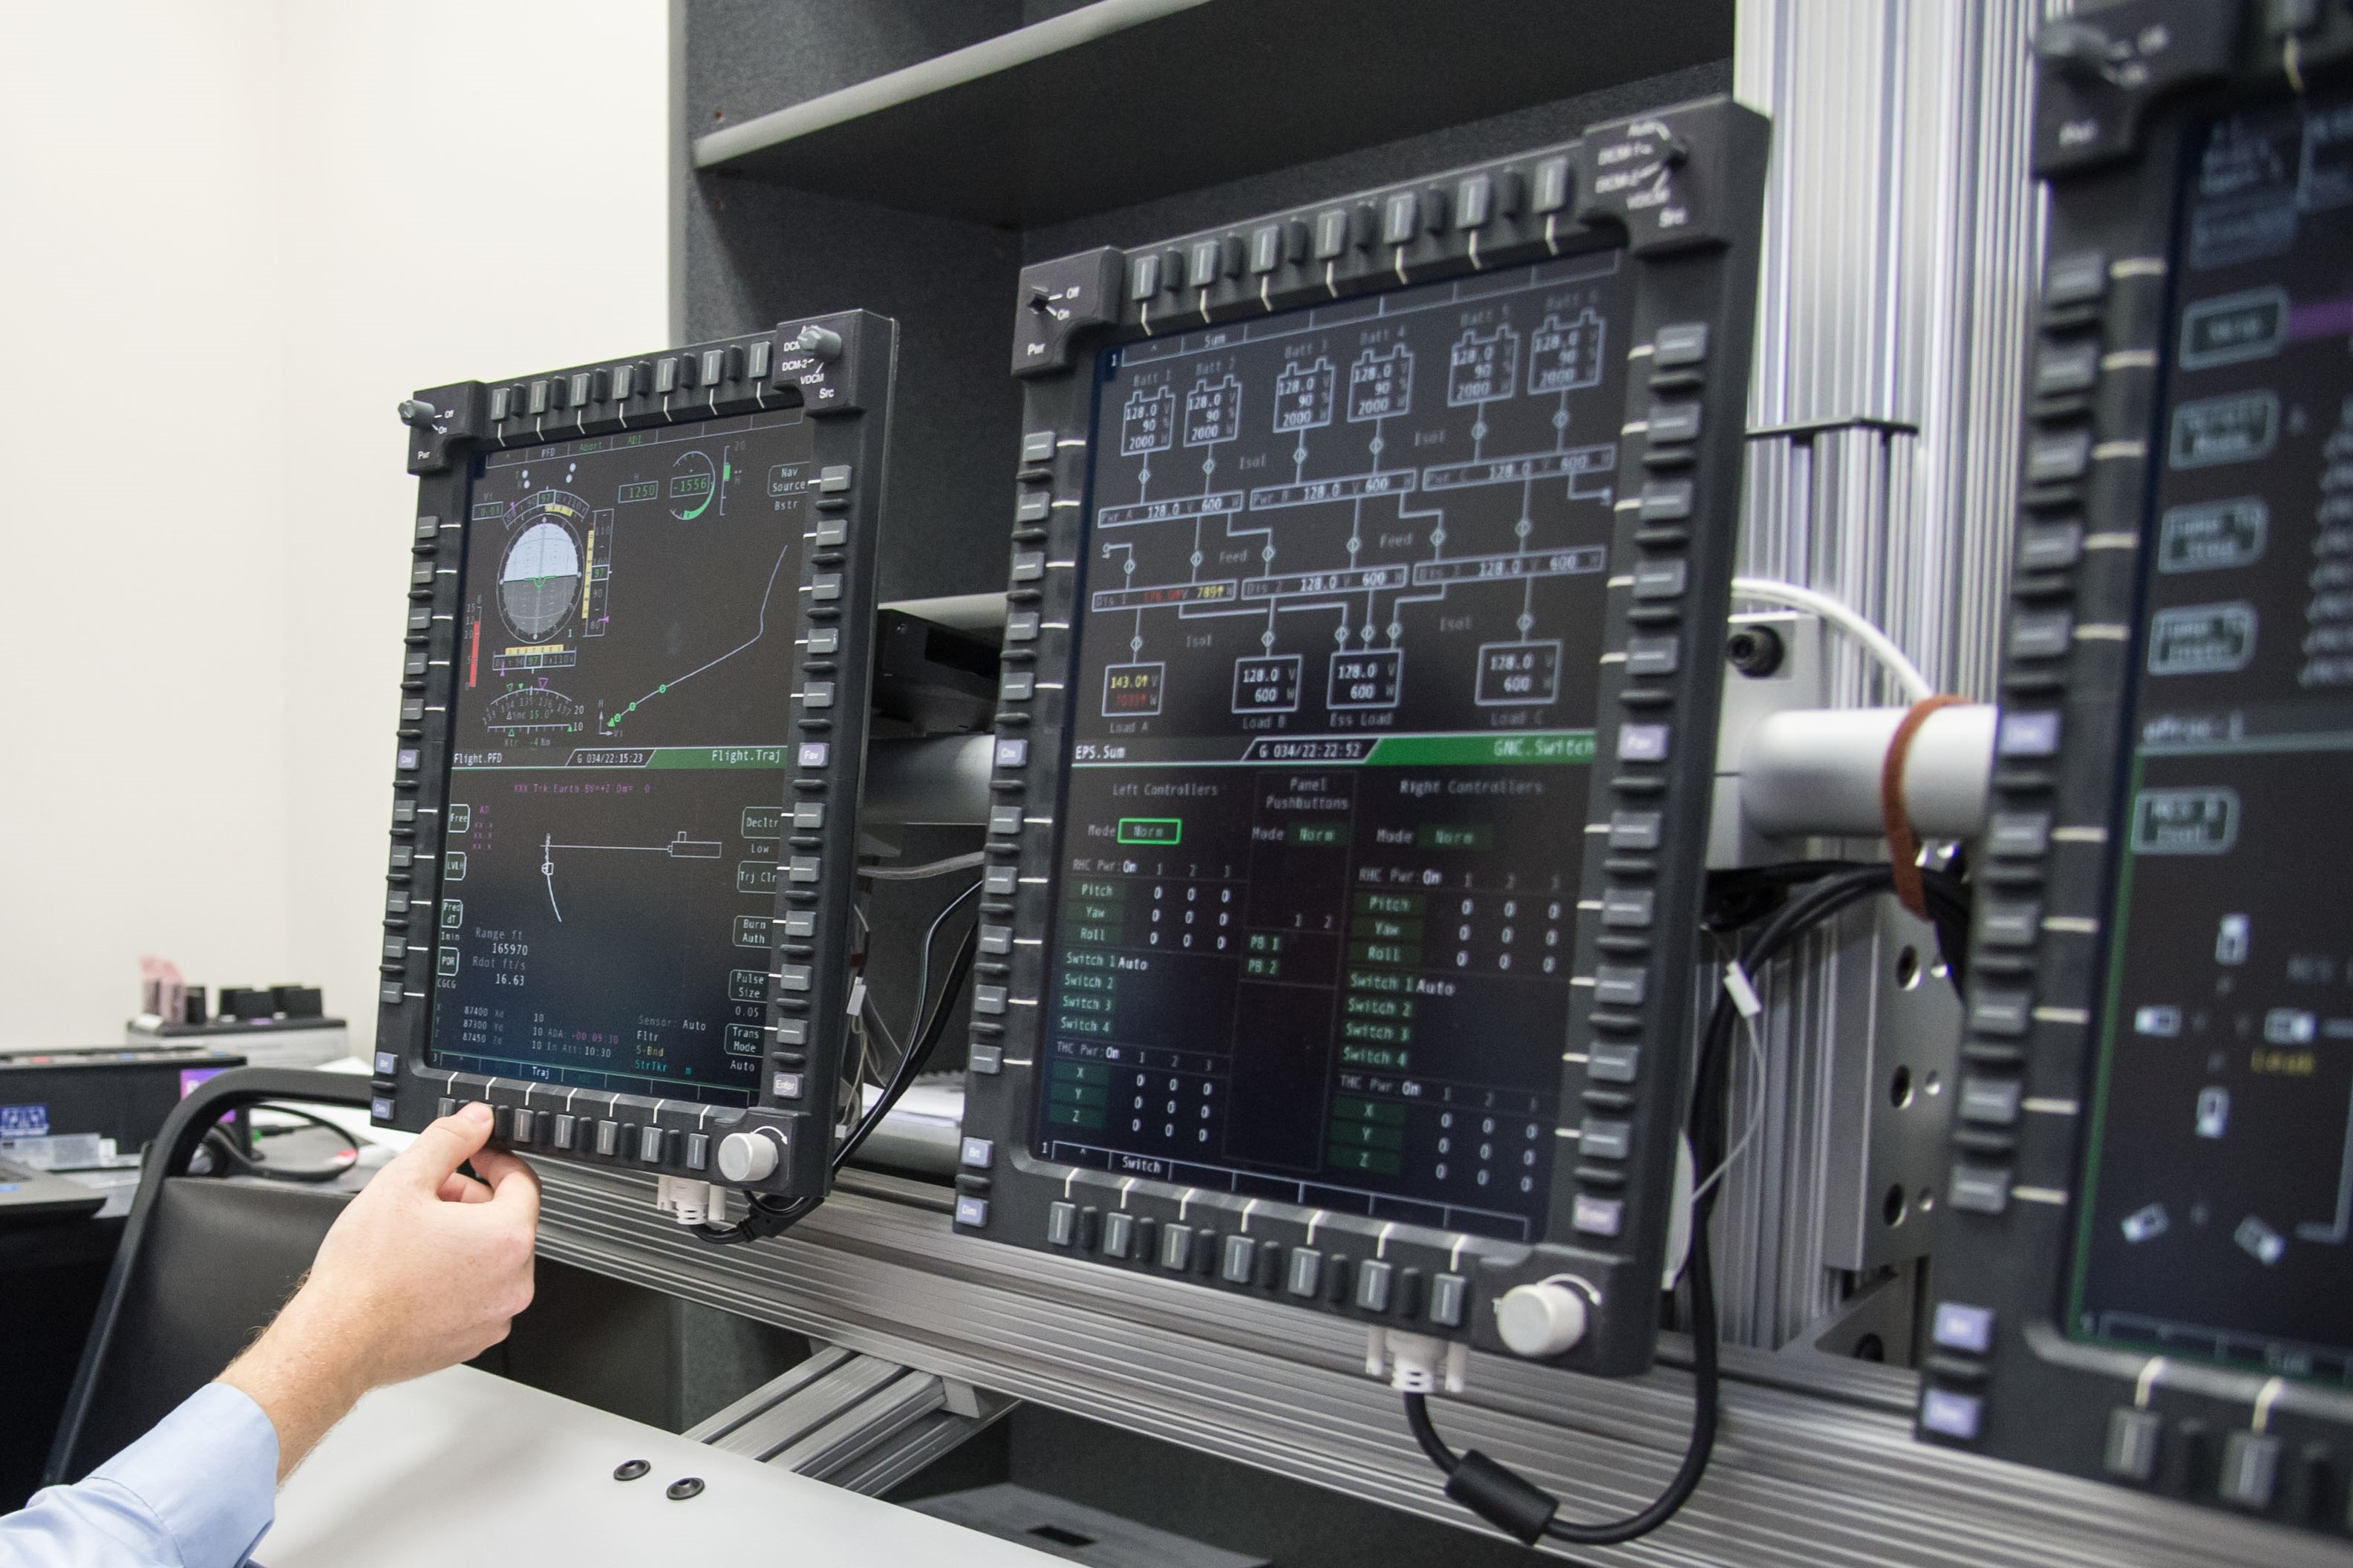
\includegraphics[width=0.9\linewidth]{orionsim.jpg}
    \caption{NASA JSC simulator of Orion cockpit instrument. The instrument design was the inspiration for our demo multifunction display instrument. Image by NASA JSC.}
    \label{fig:orion_sim}
\end{figure}

\mbox{}\hfill
\begin{figure}
    \centering
    \begin{subfigure}[t]{0.3\linewidth}
        \centering
        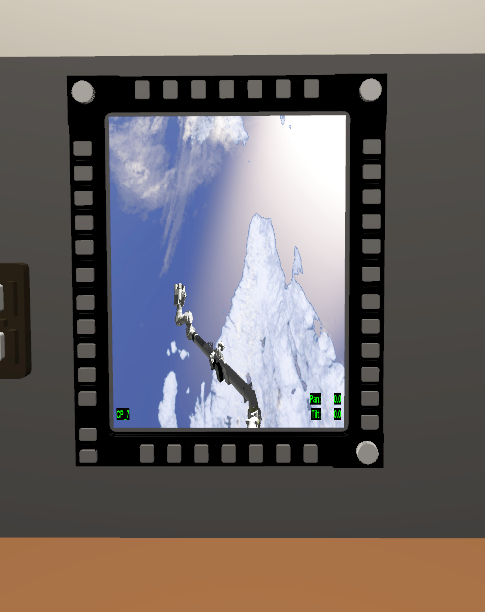
\includegraphics[width=0.9\linewidth]{proto_mfd_render.jpg}
        \caption{The MFD rendered in the virtual world.}
        \label{fig:proto_mfd_render}
    \end{subfigure}\hfill
    \begin{subfigure}[t]{0.3\linewidth}
        \centering
        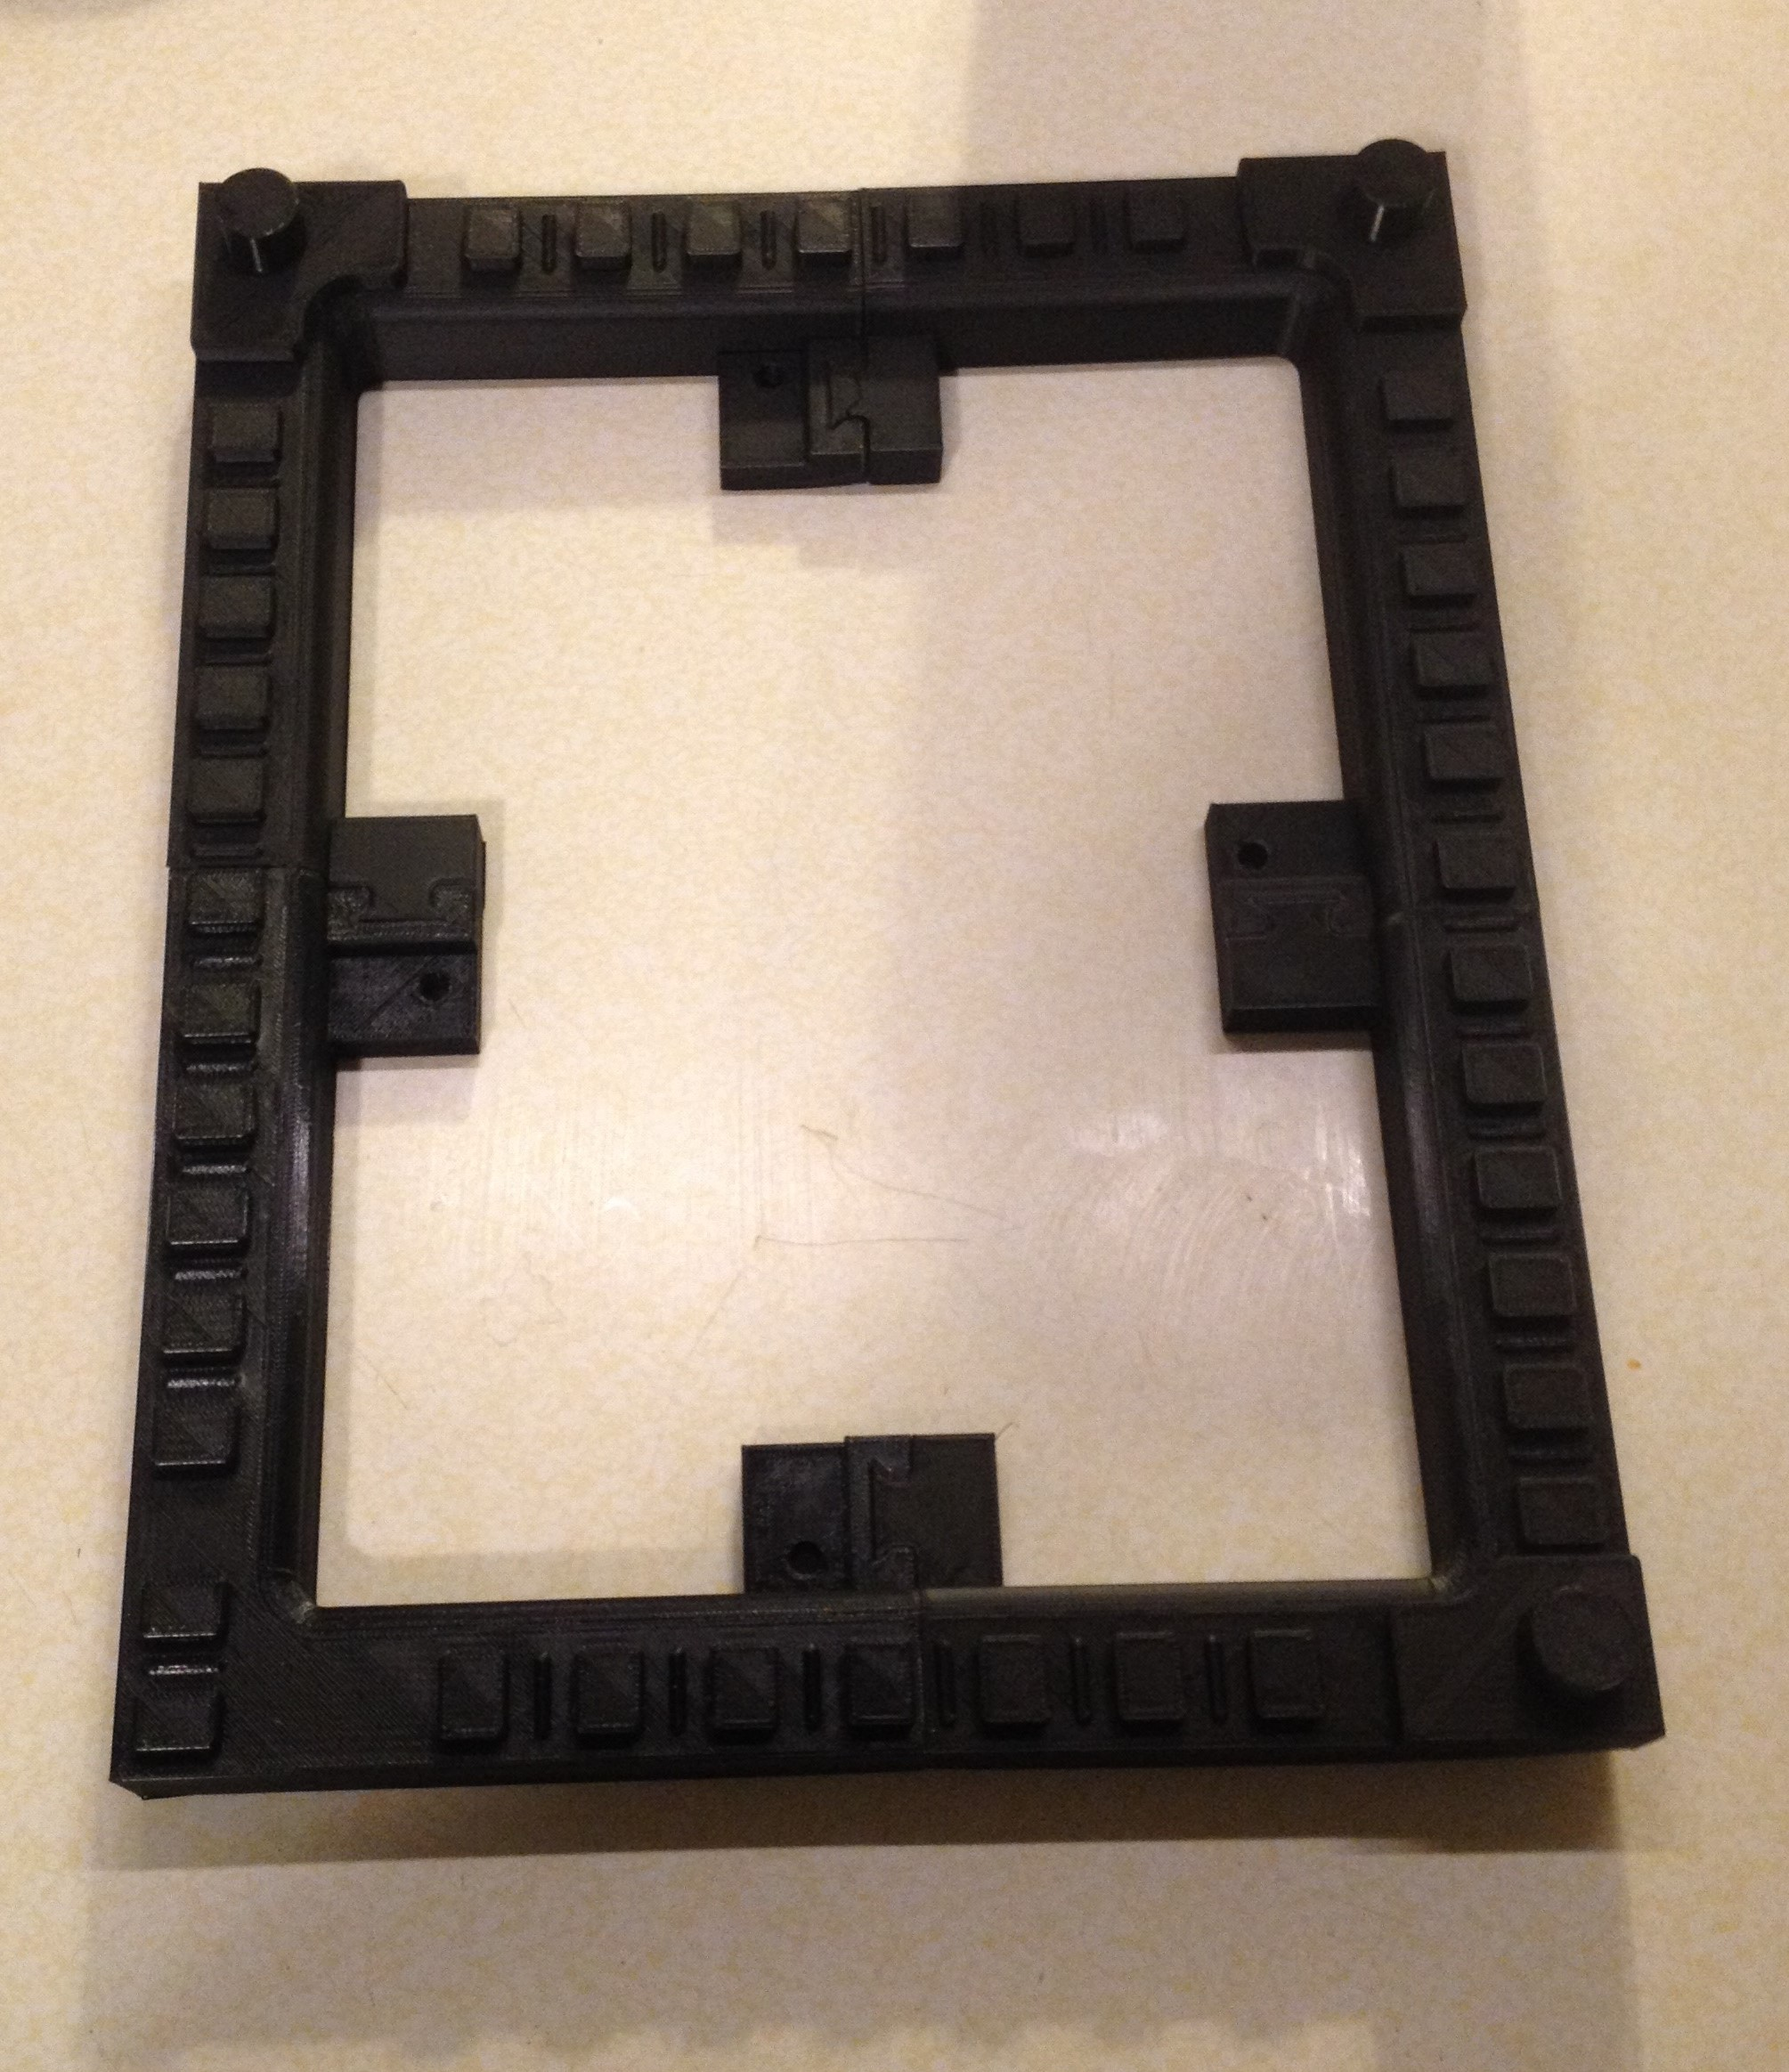
\includegraphics[width=0.9\linewidth]{proto_mfd_print.jpg}
        \caption{The 3D printed version of the MFD.}
        \label{fig:proto_mfd_print}
    \end{subfigure}\hfill
    \begin{subfigure}[t]{0.3\linewidth}
        \centering
        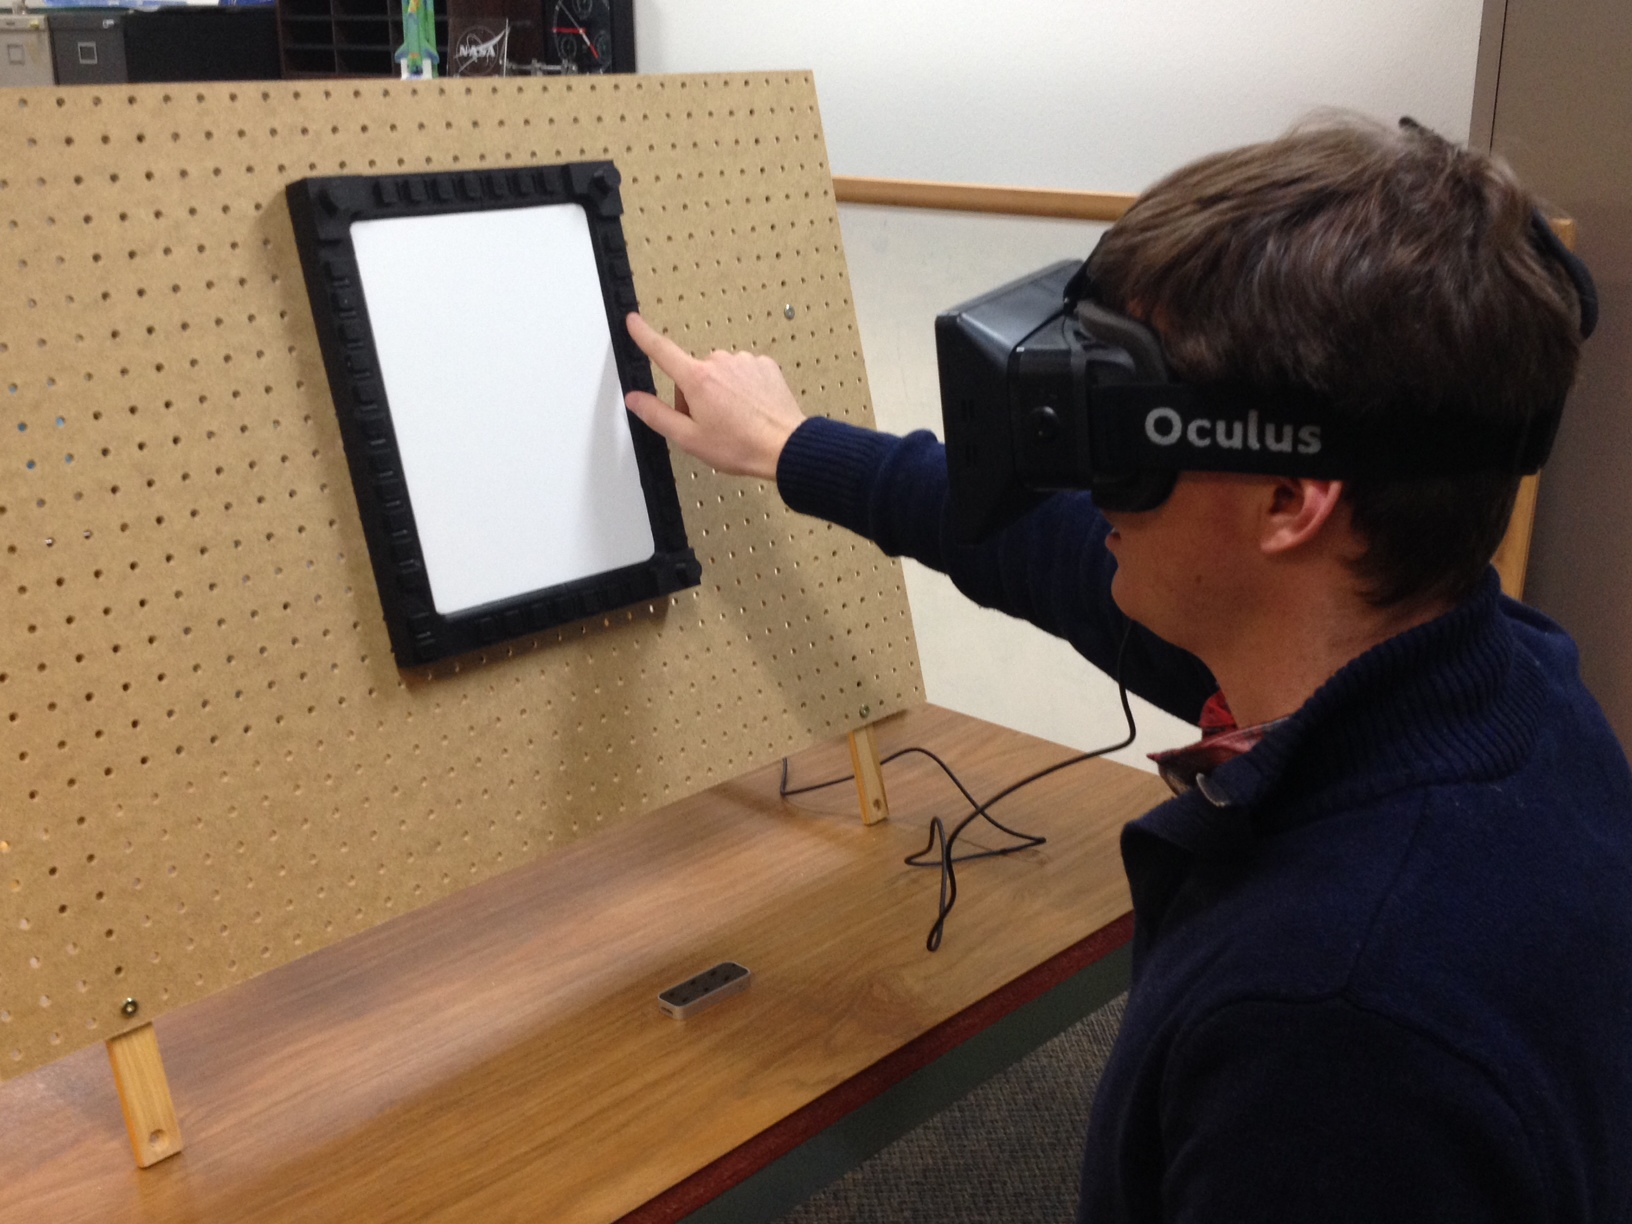
\includegraphics[width=0.9\linewidth]{proto_first_panel.jpg}
        \caption{MFD mounted on a panel.}
        \label{fig:proto_first_panel}
    \end{subfigure}
    \caption{The demo multifunction display (MFD) instrument in various configurations.}
    \label{fig:proto_mfd}
\end{figure}
\hfill\mbox{}


\subsubsection{Hand Tracking}

The LeapMotion hand tracker was selected as it provided an unobtrusive method for hand tracking.
The device itself is small (\SI{3.0 x 1.2 x 0.5}{\inch}), allowing it to be used in constrained environments (pictured in Figure~\ref{fig:proto_leap_device}).
It uses two infrared cameras to feed its proprietary tracking algorithm, and requires no gloves to be worn by the user.
The tracking volume extends rougly \num{2}~feet above the controller, and \num{2}~feet about the center on the other two axes.
This large, roughly hemispherical, field of view is shown in Figure~\ref{fig:proto_leap_fov} and can easily cover the working area of our research cockpit panel.
A larger cockpit could be supported with multiple devices.
The original version of the software, used in this prototype, provided real-time location and orientation of each fingertip.
It also gave the position and orientation of the palm, but did not provide any details on the joints or which finger of the hand the fingertip belonged to.
The tracking rate is approximately \SI{120}{\hertz}, with an advertised latency of under \num{10}~milliseconds.

\mbox{}\hfill
\begin{figure}
    \centering
    \begin{subfigure}[t]{0.49\linewidth}
        \centering
        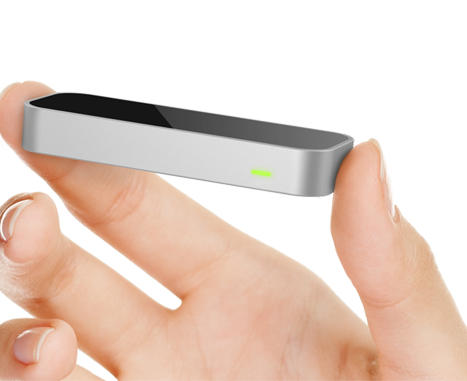
\includegraphics[width=0.9\linewidth]{leapmotion.png}
        \caption{LeapMotion device.}
        \label{fig:proto_leap_device}
    \end{subfigure}\hfill
    \begin{subfigure}[t]{0.49\linewidth}
        \centering
        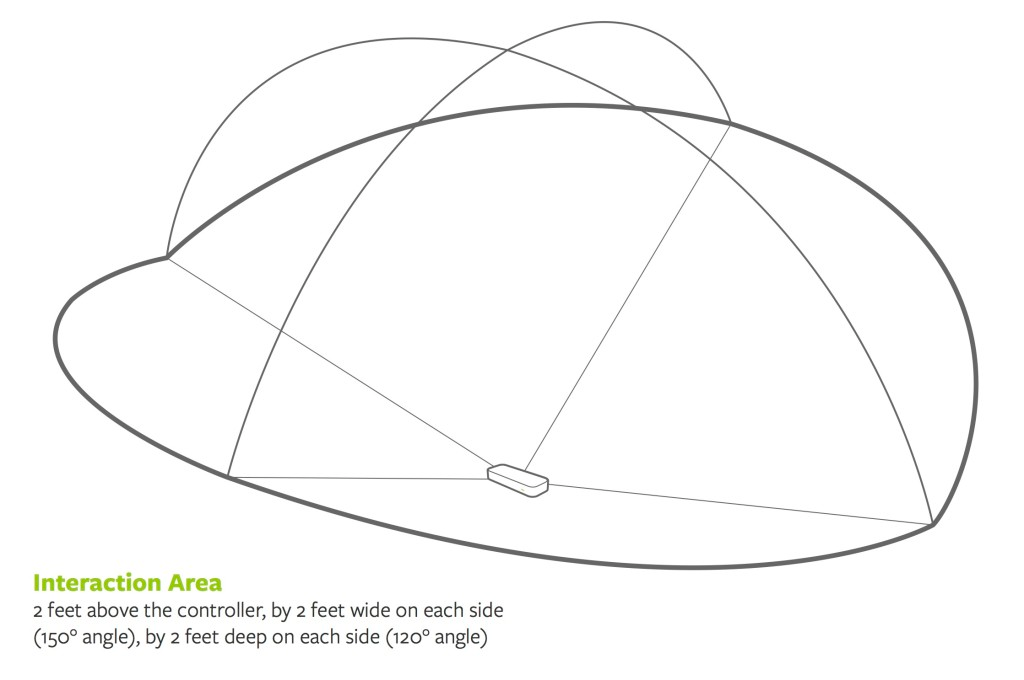
\includegraphics[width=0.9\linewidth]{leapmotion_fov.png}
        \caption{LeapMotion field of view.}
        \label{fig:proto_leap_fov}
    \end{subfigure}
    \caption{The LeapMotion device and field of view. Images by LeapMotion. Interaction area is \num{2}~feet above the controller, by \num{2}~feet wide on each side (\ang{150} angle), by \num{2}~feet deep on each side (\ang{110} angle).}
    \label{fig:proto_leap}
\end{figure}
\hfill\mbox{}

\subsubsection{Button Input Recognition}
\label{sec:proto_button_input}

Since the 3D printed buttons on the instruments are non-functioning by design, the hand tracker data needs to be used to determine when a user is ``pushing'' a button.
The 3D printed instruments do not have any movement when the buttons are pushed, so the button or key is considered activated as soon as it is touched by the users' fingertip.
The users feel the tactile feedback of the button location as they are ``pushing'' the button, and with a working button press recognition method the button would appear to work when the user touches it.

The next step was to develop the method to determine when users were touching a button using the hand tracking data from the LeapMotion.
The button recognition system was developed within the EDGE engine independent of the specific hand tracker, so that future prototypes could use a different hand tracking technology if a new device became available.

The button detection algorithm is a simple collision detection model.
A rectangular box is defined in software that extends outside the button, including a tolerance zone to account for misalignment and poor tracking.
When a fingertip enters and stays in the box for approximately \SI{150}{\milli\second}\footnote{This time is configurable and was often tweaked for each experiment.} then a button event is triggered.
The purpose of the delay is to account for false positives when a user might accidentally enter the box without intention to press the button.
The advantage to using the optical tracking to determine when a user has selected a button is that it has the potential to significantly reduce the complexity of the system.
If the user interactions with the panel can be determined solely by tracking his/her hands from the external sensor, then the cockpit panel needs only to provide physical feedback, and does not require any wiring.

\subsubsection{Challenges}

The hand tracking caused two major usability issues with the first prototype.
The first was that the reliability of the tracking caused many instances of dropped tracking, causing virtual fingers as displayed to the user to disappear unexpectedly.
The second was the conversion between hand tracker coordinates and instrument coordinates, a concept called registration.
Registration refers to the alignment between a virtual world and the real world, a concept called registration.
A well-registered virtual world will place the virutal image in a stable and precise location relative the real world.
In our application, since the virtual world is colocated with the physical componenets, having accurate registration is important to the success of the prototype.
This configuration of the prototype presented many challenges regarding registration.
Even with precise alignment of the hand tracker, the fingertip positions did not always align properly with the buttons in the virtual world.
Often, when a subject had their finger on a physical button their virtual finger was misaligned.
Since the hand tracking was not very reliable, many users would almost completely ignore its input and find the buttons by tactile feedback.
This then led to confusion when the button would not register a button press despite the strong tactile feedback.
When this occured, users would not leave the physical button to hunt for the virtual button location.

Another challenging portion of the registration was that the original version of the Oculus Rift could not measure the position of the users head relative to the real world.
This meant that the head position of the user in the virtual world was set manually.
Depending on the actual position of the user, the panel would not appear with the correct scale and at the correct distance in the virtual world.
This caused users to initially reach too short or too far for the panel, and decreased the realism as the panel seemed too small or large compared to the real world object.
Since the head tracking sensors were all internal to the headset, it also experienced drift after a few minutes.
Most noticeable in the yaw, it would cause the panel to become misaligned and require a manual reset to realign.

\subsection{Second Prototype}

A number of improvements were made in the second generation of the prototype.
Due to vendor provided software upgrades, the hand tracking became more robust and provided more complete information about the entire hand position.
The visuals were upgraded with the second Development Kit of the Oculus Rift, which provided improved visual resolution, but, more importantly, an external head tracker (using an infrared camera) which enabled accurate detection of head movement and virtually eliminated drift of the internal intertial sensors.
A major focus of this version of the prototype was to improve reliability and registration.
The reliability was partially improved with the new hand tracking software, but other countermeasures developed are described as well.
Registration (the alignment between the physical world and the virtual world) was improved with the use of a new calibration mechanism described in this section.

\begin{figure}
    \centering
    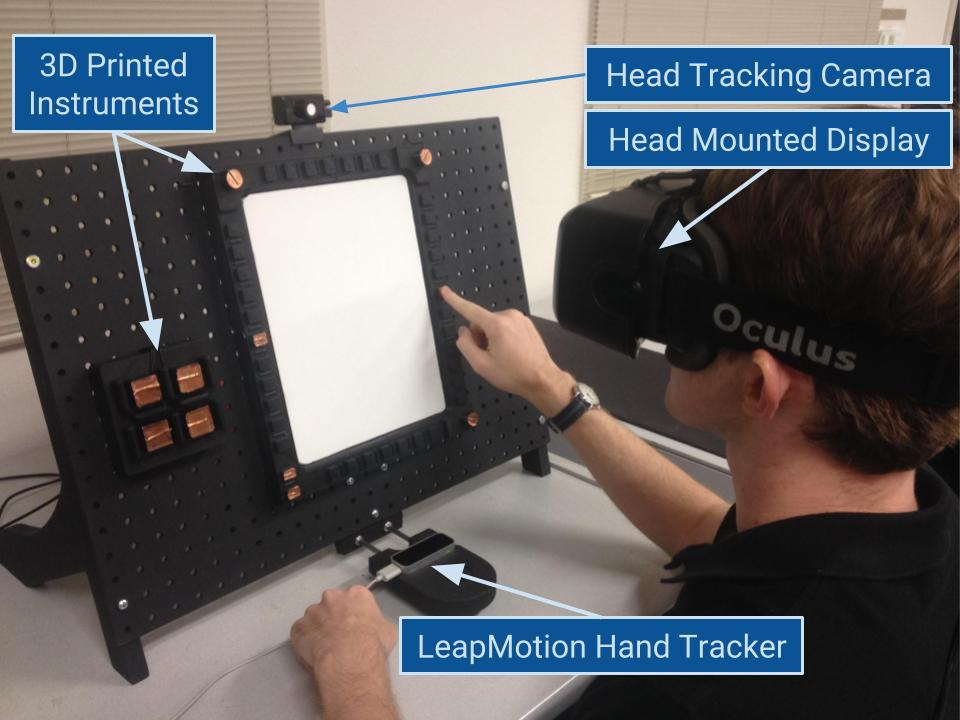
\includegraphics[width=\linewidth]{r3c_callout.jpg}
    \caption{A version of the second prototype with major components noted.}
    \label{fig:r3c_callout}
\end{figure}

\subsubsection{Virtual Reality Headset}

The head tracking provided in the second Oculus Rift development kit version gave a significant improvement over the original version in the registration between the real world and the virtual world.
Now with the head fully tracked with positional updates, the user can more freely explore the virtual world.
With the original Oculus Rift, the location of the head was fixed in the virtual world and only orientation was provided.
The head positional tracking follows the movement of the head from side to side or back and forth, providing a more immersive experience to the user.
This provides the user with additional parallax depth cues to better gauge the size and distance of objects.

The position and orientation of the user's head is reported relative to the tracking camera which is placed facing the user.
The camera can be mounted in a well-known location relative to the panel which provides a head position in the virtual world precisely measured relative to the panel.
This means the virtual world is rendered with a more correct eyepoint of the user compared to the first version.
The virtual components are now always rendered at the correct distance and with proper scale.
The head-tracking camera is shown mounted on the instrument panel in Figure~\ref{fig:r3c_callout}.


\subsubsection{Hand Tracking}
\label{sec:proto-hand-tracking}

The upgrade to the LeapMotion hand tracking software provided two integrated features.
The first feature was an improvement in the fidelity of the tracking, including full information on the joints of the hand.
The second was the introduction of a ``head-mounted'' mode, which allowed for tracking to be optimized for looking down at a hand.

The tracking upgrade added the location and orientation of the entire hand at a skeletal level.
This means all the joints and the bones between them are tracked.
The upgraded view is shown in Figure~\ref{fig:proto_skeleton}.
This provided a more immersive feeling than the floating fingers of the original LeapMotion software used in the first prototype.

\begin{figure}
    \centering
    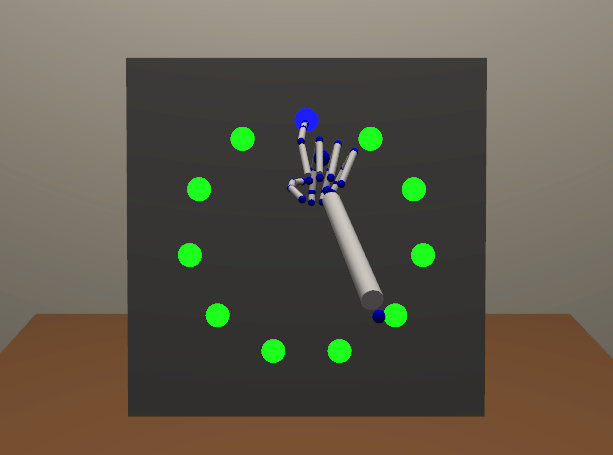
\includegraphics[width=\linewidth]{leap_skeleton.png}
    \caption{The complete hand tracking of the LeapMotion v2 software.}
    \label{fig:proto_skeleton}
\end{figure}

At the same time of the tracking upgrade, a ``VR Mode'' was introduced to the LeapMotion software to provide hand tracking in a virtual environment by way of mounting it on the head-mounted display itself.
Upon initial testing of this feature, two observations were made.
The tracking was improved with a perspective looking down at the hands, instead of being below looking up at the palms of the hands.
This configuration seemed to provide more robust and reliable tracking data.
Using it mounted to the head-mounted display, however, caused a large issue with the registration between the real and physical world.
The registration between the hand tracker and the location of the instruments relies on a known, rigid connection.
When the tracker was mounted on the head-mounted display, the transformation between LeapMotion coordinates and panel coordinates relied on knowing the location of the head.
Although this information could be obtained from the newer model HMD which included head tracking, it was not precise or stable enough to use as the base for the hand tracking coordinates.
For example, if a hand was placed resting on the panel and kept still, the virtual hand would appear to move relative to the virtual panel if the head were moved at even a moderate pace.
The additional latency introduced by relying on the head tracking sensors simply would not keep accurate registration.
This led us to develop a mount that would hold the LeapMotion upside down, looking down over the panel and instruments (Figure~\ref{fig:proto_leap_mount}).
The software could still be configured to the ``VR Mode'', optimizing for face-down tracking, but with a rigid mount.
This provided the best of both worlds: the reliability of the camera down tracking, and a stable transformation between the tracker coordinates and the panel coordinates.

\begin{figure}
    \centering
    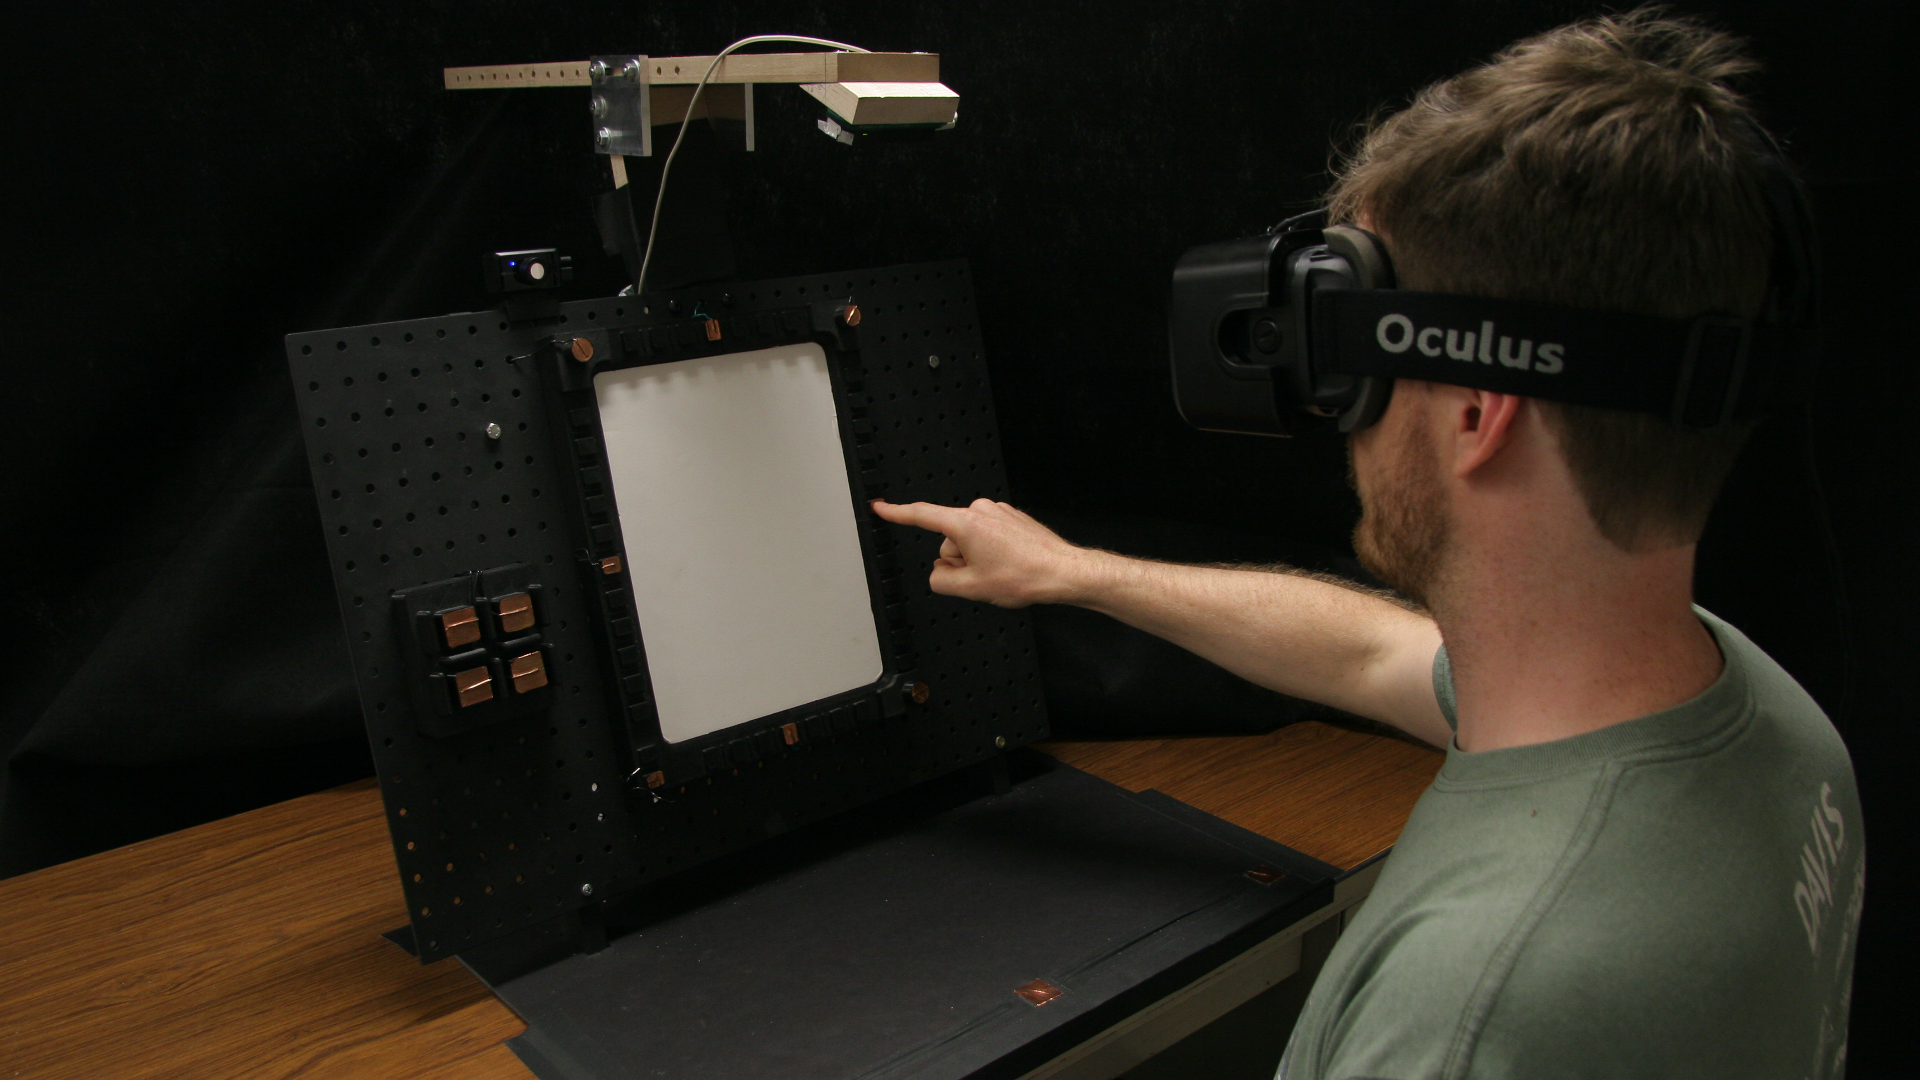
\includegraphics[width=\linewidth]{leap_mount.jpg}
    \caption{The LeapMotion mount, holding the sensor above the panel and looking down.}
    \label{fig:proto_leap_mount}
\end{figure}

\subsubsection{Button Recognition Countermeasures}

Two countermeasures were introduced in this prototype that aided new users in learning the button recognition algorithms of the hand tracker.
A simple visual indication was added when a user entered the detection box in front of the button.
This was typically implemented with the button itself being highlighted or changing color.
With this crucial feedback, new users were able to learn the tolerances of the button zone and understand when the button was going to be activated.
For experienced users, the feedback provided confirmation that they were in the zone and were not waiting for it to register incorrectly.
The second countermeasure was the addition of an aural feedback upon the button press being registered.
Instead of relying solely on visual feedback, the addition of a ``click'' noise when the button press was registered allowed the user an additional way to confirm the action of the button press had properly registered.
This was especially helpful when the user became familiar enough to register buttons with their peripheral vision as they could use the audio feedback to know the button had been pressed.
These two countermeasures for the difficultly of working with the button recognition were observed as being very helpful to new users, and were included in all versions of the prototype used for the research studies.

\subsubsection{Capacitive Touch Sensors}
\label{sec:proto_cap_touch}

In order to be able to activate the buttons reliably when the hand tracking was degraded or dropped out, the use of capacitive touch sensors was investigated.
The capacitive touch sensors were initially developed as a countermeasure to the problems encountered with the hand tracking from the original prototype.
As the hand tracking became more robust with the new software from the manufacturer, however the countermeasure was not as important, but the sensors played a new role in the prototype: validating the accuracy, and providing calibration for the hand tracker.

With the requirement of minimal setup, the original capacitive touch sensors were developed with copper tape electrodes placed on the top of the 3D printed instrument buttons.
These electrodes are shown on the demo multifunction instrument in Figure~\ref{fig:copper_pads}.
A Freescale MPR121 capacitive touch sensor was used to read the electrodes and communicate with an Arduino which sent touch events over a serial communication line to the computer.
These serial events were read by the rendering engine to trigger events when a copper pad was touched.
These simple, single electrode per button sensors provided a reliable method for determining when the user had actually touched a button.
The main use of these sensors evolved to be for the calibration mechanism described in the next section.
However, as the registration improved, a research question was developed around how accurately the user could place a fingertip on the physical button while immersed visually in the virtual world.
This led to the development of a second generation of capacitive touch buttons, used in the Pointing Experiment (Chapter~\ref{chap:pointing}).

\begin{figure}
    \centering
    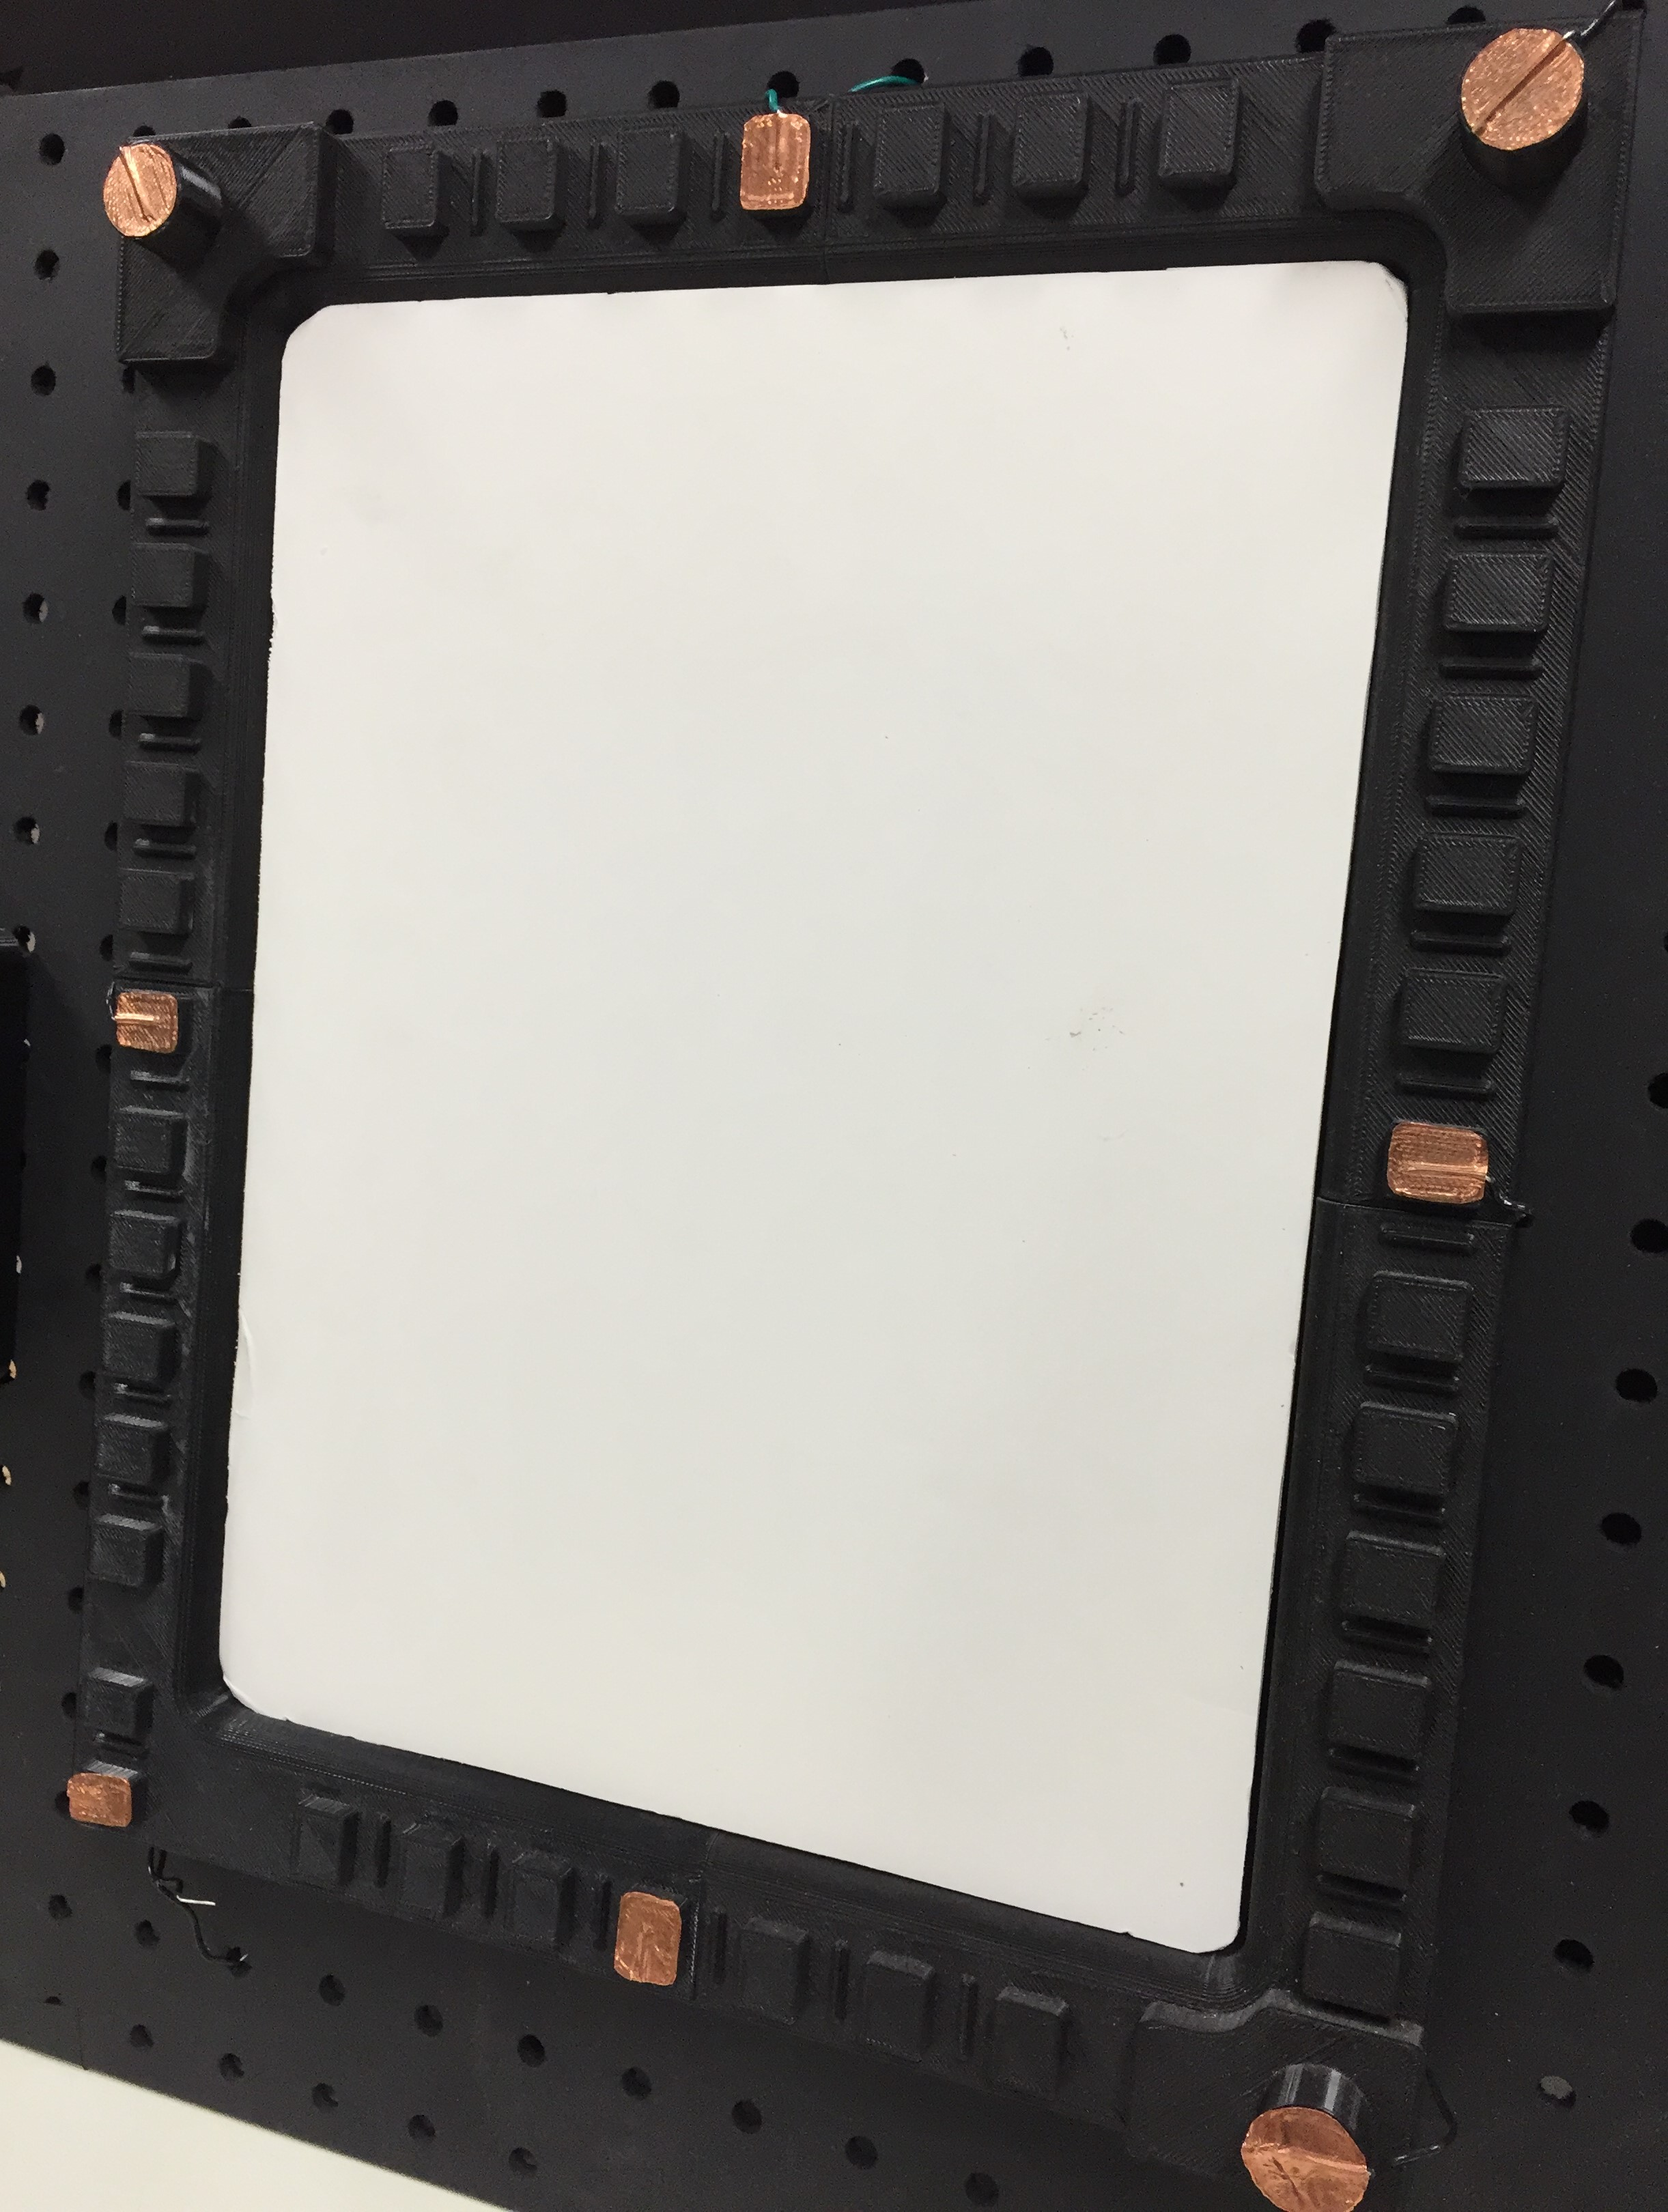
\includegraphics[width=0.5\linewidth]{copper_pads.jpg}
    \caption{The copper tape electrodes for capacitive touch sensors on the demo multifunction instrument.}
    \label{fig:copper_pads}
\end{figure}

Since touch accuracy can be important in safety-critical applications, we developed the ability to record where on the button the finger press was located using a capacitive touch sensor.
To accomplish this, a custom printed circuit board was developed that provides an electrode array of 5 rows and 5 columns over a 1-inch by 1-inch square.
This board is shown in Figure~\ref{fig:proto_capacitive_array}.
The capacitive state of each row and column can provide a measurement of the center of the finger press on the grid created by the rows and columns.
The center of the finger press location can be found with an accuracy of under 0.1-inch using this configuration.
The location of the finger press can help provide a measure of the accuracy of the registration between the optical sensors and the real world location, as well as any bias introduced from using the VR headset and hand tracker.

\begin{figure}
    \begin{subfigure}[t]{0.32\linewidth}
    \centering
    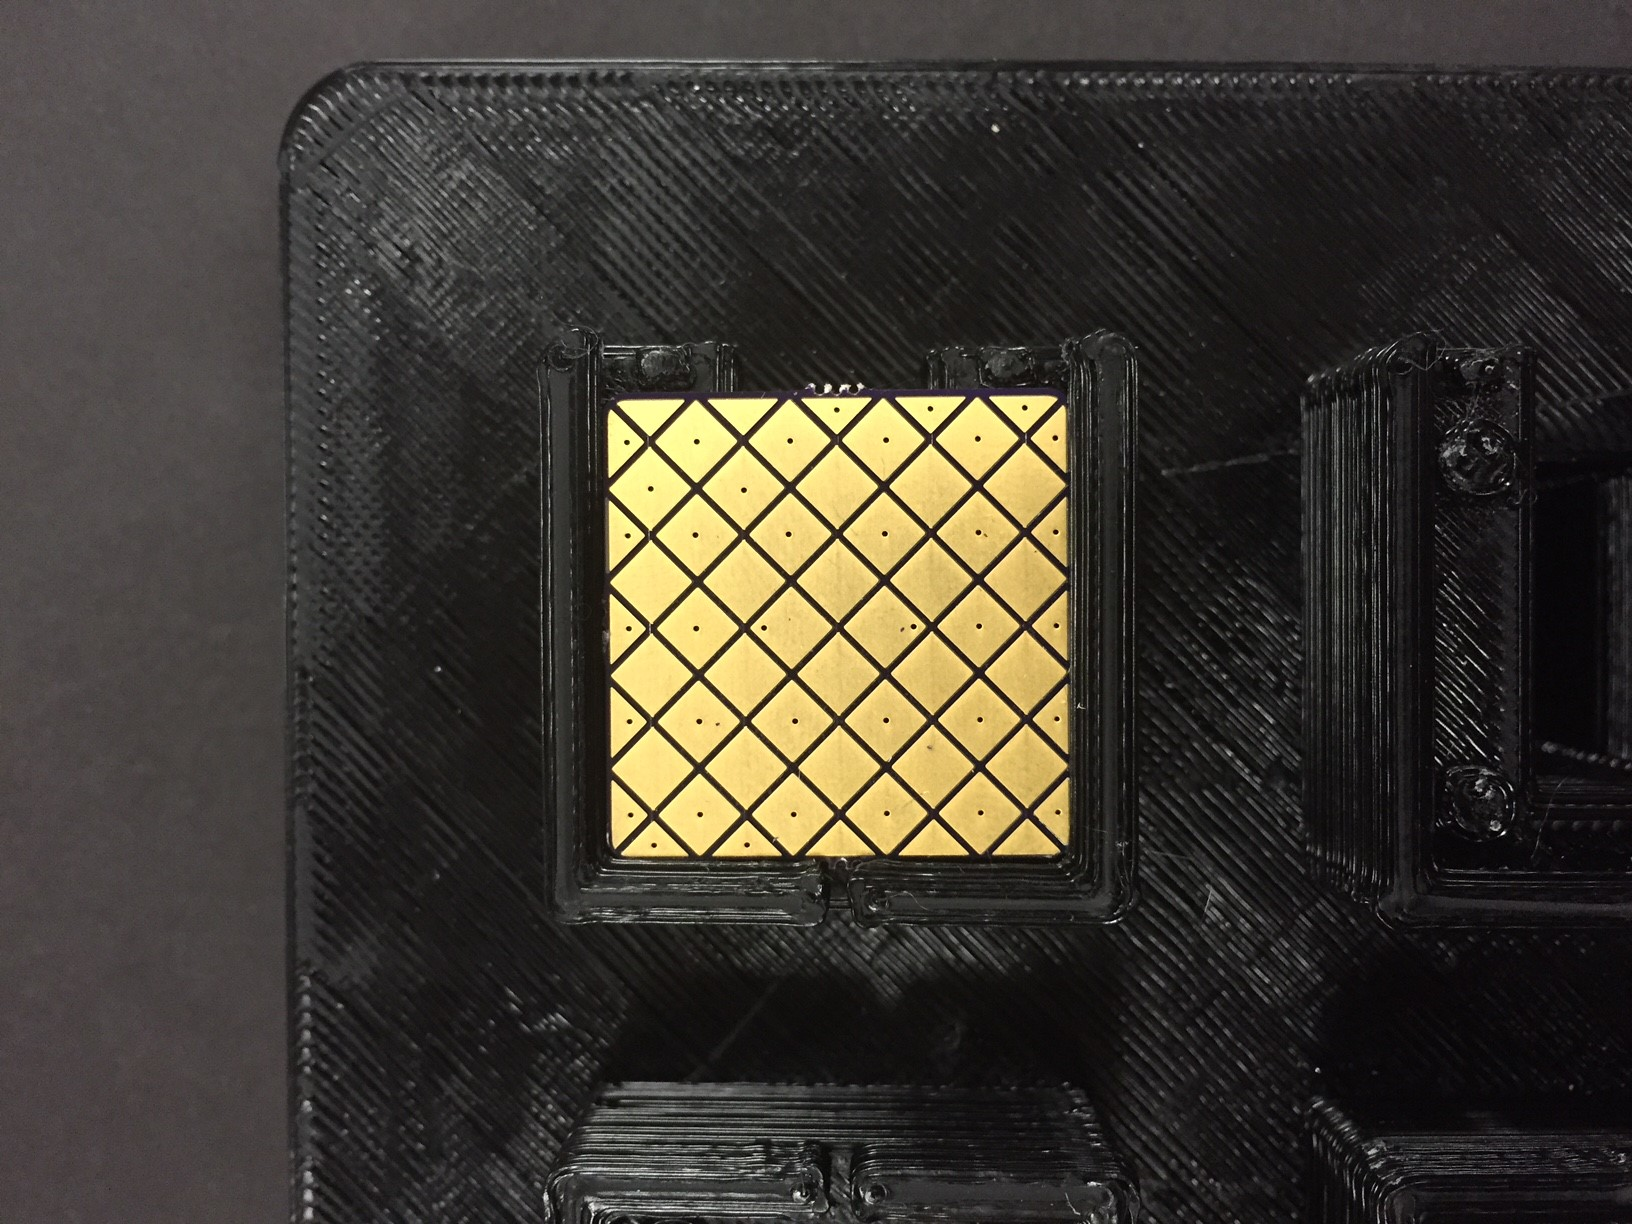
\includegraphics[width=1.5in]{pe_capacitive.jpg}
    \caption{Capacitive array mounted in a 3D printed button.}
    \label{fig:proto_capacitive_array:mounted}
    \end{subfigure}
    \begin{subfigure}[t]{0.64\linewidth}
    \centering
        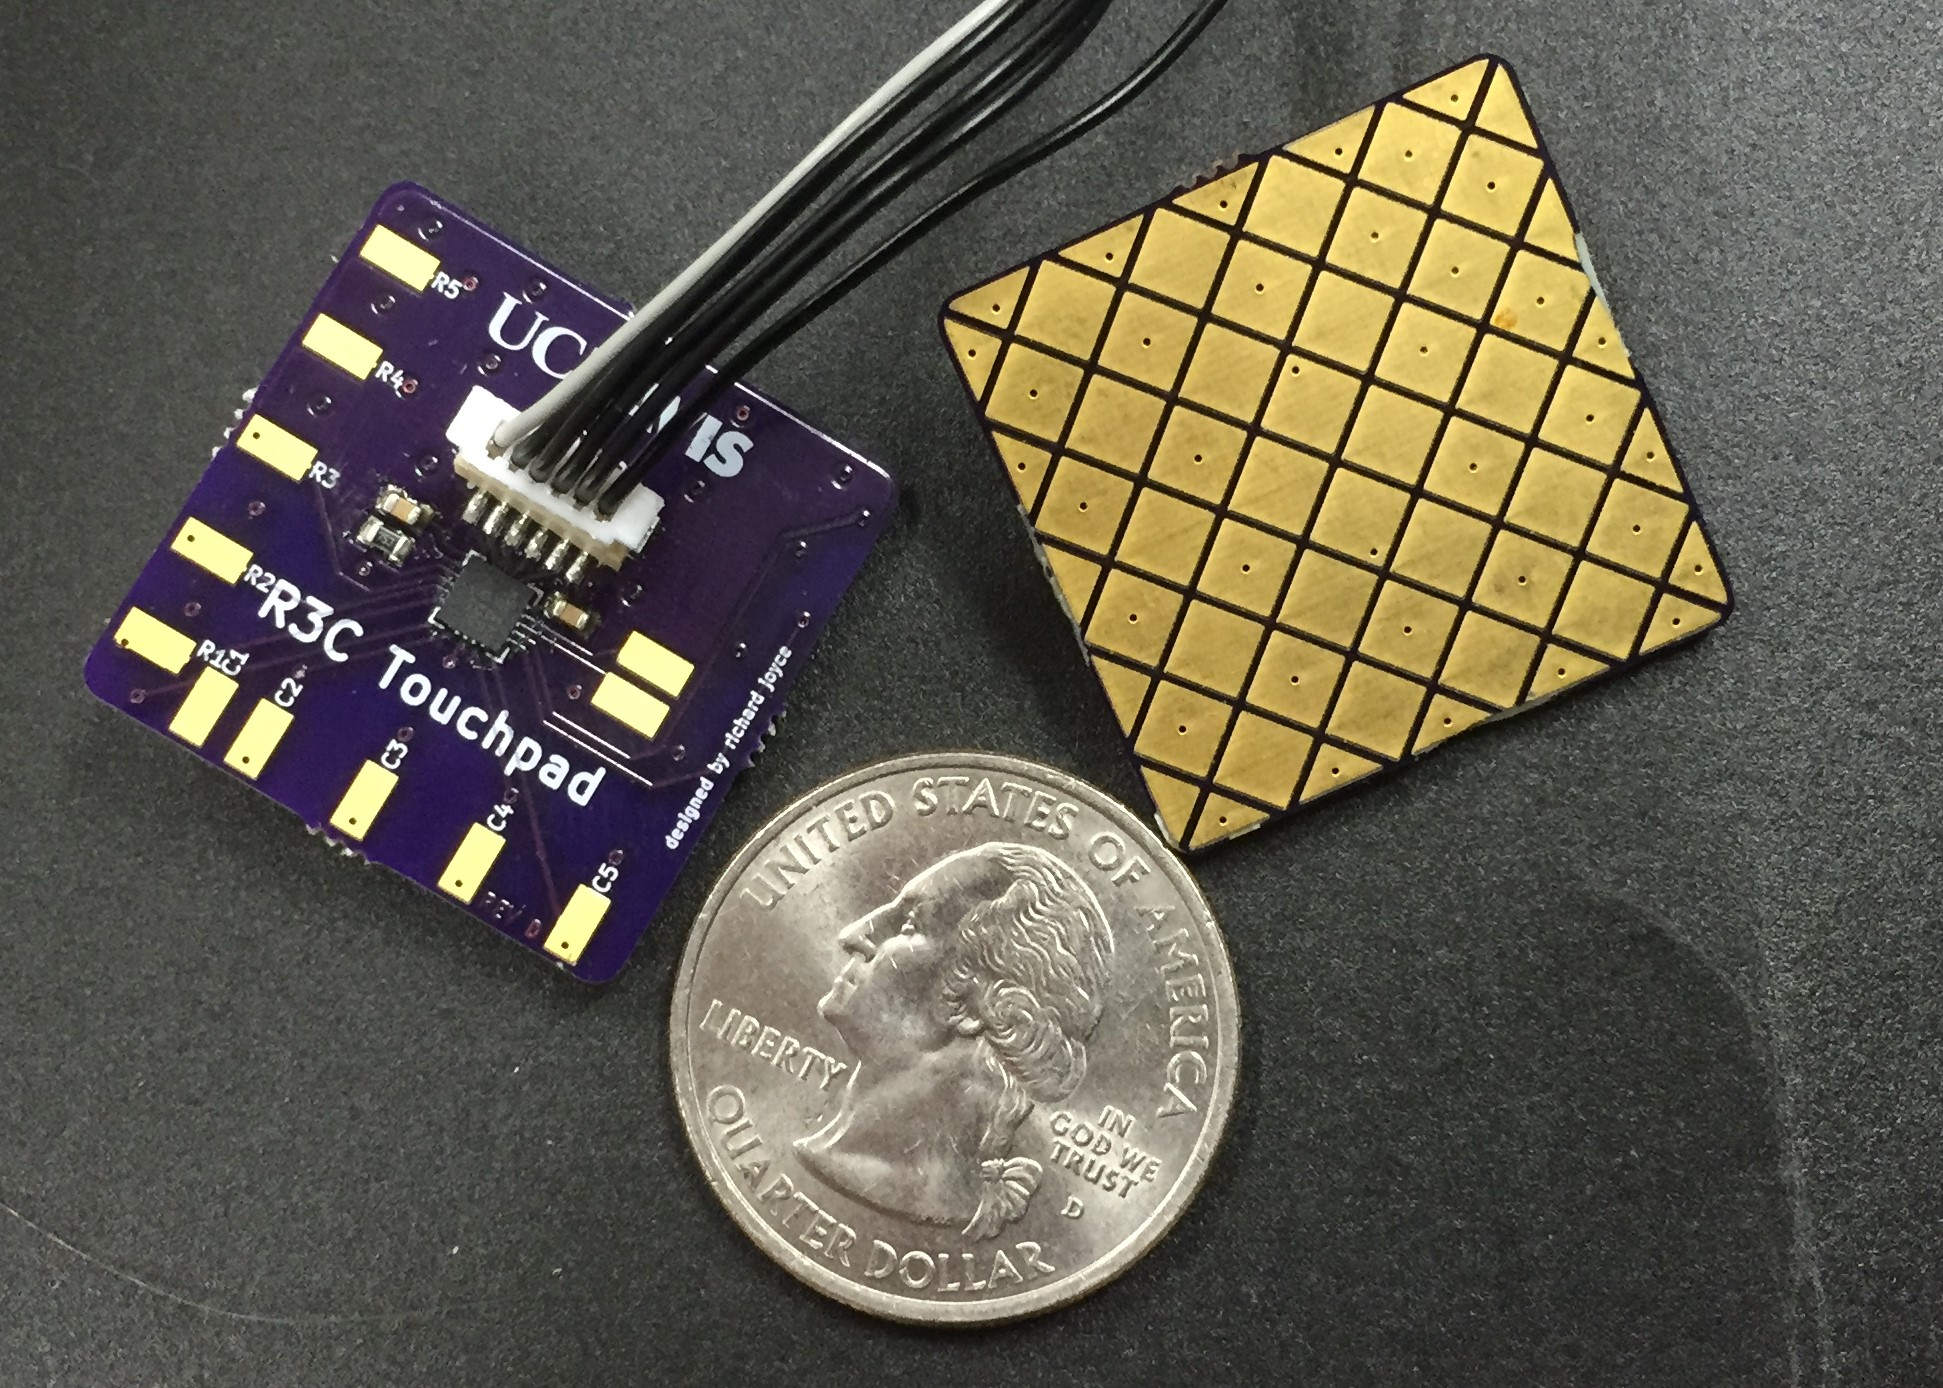
\includegraphics[width=\linewidth]{proto_cap_board.jpg}
    \caption{Bare PCB showing back and front.}
    \label{fig:proto_capacitive_array:pcb}
    \end{subfigure}
    \caption{Capacitive touch array button. Each row and column of diamond pads are connected as one electrode each and together can provide location information of where the user presses.}
    \label{fig:proto_capacitive_array}
\end{figure}

\subsubsection{Calibration}
\label{sec:proto-calibration}

The hand tracking of the LeapMotion was observed in pilot studies to provide precise and repeatable measurement of the hand positions throughout its tracking volume.
However, the accuracy was observed to be insufficient.
Put another way, the position of a finger on the button in the physical world was shown offset from the button position in the virtual world, yet the offset was consistent between movements.
This error also increased as the finger moved from buttons close to the sensor to buttons further from the sensor.
This led us to develop a calibration to provide a more accurate registration between the virtual and physical hand positions.
With the addition of the capacitive touch sensors, a calibration mechanism was developed with the use of the known positions in the physical world (the capacitive touch sensor locations).
This means that when a finger was placed on a physical button with a capacitive sensor, the known position can be recorded along with the ``measured'' position of the hand tracker.
After collecting enough points, the calibration can correct for the measured offset and provide an accurate registration between the real and virtual worlds.
The mathematical basis for this calibration is described here.

The calibration works on the assumption that there exists a transformation matrix, $\mathbf{T}$, that can solve the following equation:
\begin{equation}
    \vec{x}_{known} = \mathbf{T}\vec{x}_{measured}
    \label{eq:proto_Tvec}
\end{equation}
The $\vec{x}_{known}$ and $\vec{x}_{measured}$ correspond to the known location of a calibration point (button) and the location measured by hand tracker, respectively.
Since we know those two vectors, it is only required to solve for the transformation matrix itself.

A simple least squares approach is used to find the coefficients of the matrix. % the registration between the virtual and physical worlds is vastly improved.
The transformation matrix is not constrained to a simple rotation (i.e.\ not assumed orthogonality or other special properties) so the solution is found by expanding and solving the general homogeneous coordinates transformation matrix.
\begin{equation}
    \begin{bmatrix}
        x_{known} \\
        y_{known} \\
        z_{known} \\
        1
    \end{bmatrix} =
    \begin{bmatrix}
        T_{11} & T_{12} & T_{13} &T_{14} \\
        T_{21} & T_{22} & T_{23} &T_{24} \\
        T_{31} & T_{32} & T_{33} &T_{34} \\
        0 & 0 & 0 & 1
    \end{bmatrix}
    \begin{bmatrix}
        x_{measured} \\
        y_{measured} \\
        z_{measured} \\
        1
    \end{bmatrix}
    \label{eq:proto_Tmat}
\end{equation}

Typical least squares approaches would attempt to find $\vec{x}_{measured}$ in Eq.~\ref{eq:proto_Tvec}, however we desire to find the matrix $\mathbf{T}$ itself.
It can be shown that expanding the matrix equation (Eq.~\ref{eq:proto_Tmat}) for the multiple calibration points (i.e.\ $\vec{x}_{known,1},\dots,\vec{x}_{known,n}$ and $\vec{x}_{measured,1},\dots,\vec{x}_{measured,n}$) and then collecting like terms will convert the problem into three different least squares problems.
They are shown here with subscripts $k$ and $m$ for `known' and `measured'.

\begin{gather*}
    \begin{bmatrix}
        x_{k1} \\
        x_{k2} \\
        \cdots \\
        x_{kn}
    \end{bmatrix}
    =
    \mathbf{X}_M
    \begin{bmatrix}
        T_{11} \\
        T_{12} \\
        T_{13} \\
        T_{14}
    \end{bmatrix}
    ,\;\;
    \begin{bmatrix}
        y_{k1} \\
        y_{k2} \\
        \cdots \\
        y_{kn}
    \end{bmatrix}
    =
    \mathbf{X}_M
    \begin{bmatrix}
        T_{21} \\
        T_{22} \\
        T_{23} \\
        T_{24}
    \end{bmatrix}
    ,\;\;
    \begin{bmatrix}
        z_{k1} \\
        z_{k2} \\
        \cdots \\
        z_{kn}
    \end{bmatrix}
    =
    \mathbf{X}_M
    \begin{bmatrix}
        T_{31} \\
        T_{32} \\
        T_{33} \\
        T_{34}
    \end{bmatrix}
    ,\\
    \text{where}~\mathbf{X}_M =
    \begin{bmatrix}
        x_{m1} & y_{m1} & z_{m1} & 1 \\
        x_{m2} & y_{m2} & z_{m2} & 1 \\
        &\dots & & \\
        x_{mn} & y_{mn} & z_{mn} & 1
    \end{bmatrix}
\end{gather*}

Now the problem is stated with a known matrix and one unknown vector (per each of the three equations).
Once we have collected more than 4 points, it becomes an over-determined linear system, and a least squares calculation is used to find the solution.
From the solution of the three separate equations, the original $\mathbf{T}$ matrix is reconstructed.

At least 4 points are needed to solve this system, and it has been found that a calibration with small least squares residuals can be achieved with 10-20 well chosen points.
Provided no changes to the lighting or the position of components, the calibration setup can be performed once for the setup and works across users.

Instead of using the calibration matrix, $\mathbf{T}$, to transform all of the points in the hand, the index finger was used as the datum for the calibration.
The offset of the index finger between the measured and calibrated positions was calculated and then the entire hand was offset by this vector.
This was done as it was quickly observed that significant and unrealistic warping occurs with the virtual hand if all points are transformed with the calibration matrix.
This kept the relative position of each joint in the hand as reported by the LeapMotion while calibrating against the point that was most frequently used for button targeting\footnote{Subjects in all research studies were instructed to use their index finger.}.

\subsubsection{Lessons Learned}

The capacitive touch sensors used to activate the buttons were found to be effective.
However, they added additional complexity to the hardware setup of the R3C system.
The calibration mechanism developed created a more accurate registration that enabled button activation without the capacitive touch sensors.
The difference in using the capacitive touch sensors and the hand tracking only to activate buttons was investigated in the first research study, detailed in Chapter~\ref{chap:pointing}.
Before the calibration working to improve registration, new users would rely on the physical feedback and wait for the button registration with their finger on the physical button, despite the visuals showing them their finger misaligned in the virtual world.
A more experienced user, knowledgeable about the method of button detection, would know to ignore the physical feed and move to find the detection zone by aligning the finger with the virtual button and not the physical button.
Additionally, we discovered that hand pose and speed of movement can influence the performance of the hand tracker, and that more experienced users tended to learn techniques that gave the hand tracker a reliable measurement.
For example, when the tracker was first acquiring the hand (from outside the field of view), having the fingers spread out led to a quicker acquisition time for the tracker.
Providing the hand tracker with a good angle to view the hand at all times was something that experienced users learned as well.
We often found that a small amount of training time would greatly improve performance.

Not all of the input interactions with a cockpit may be measurable with just optical tracking.
Some interactions which require a fast reaction time or dynamic input (i.e.\ flight control manipulation) may not be suitable with the current technology.
These observations are investigated throughout the research studies, and help to quantify which tasks may be appropriate for this type of prototyping system.

With this prototype it was initially noticed that the tracking performance became less reliable and would often drop out as the hand approached the panel and instruments.
This was particularly frustrating for users as it was precisely where the hand tracking was needed the most as it was needed to activate the button.
After isolating the problem to the presence of the panel and instruments, it was discovered that we had inadvertently provided optical interference to the hand tracker.
When looking at the raw image captured by the LeapMotion infrared cameras we found that our glossy black 3D printed instruments were highly reflective in infrared, causing little to no contrast between the hand and the instruments.
Applying a matte paint finish improved this, and the reflections in infrared were monitored for future prototypes and configurations.
We have also found better results when covering the entire backdrop of the LeapMotion field of view with a dark matte material, as this helps provide a greater contrast between the hand and the background.


\subsection{Third Prototype}

The third prototype was developed for the design evaluation experiment.
The motivation for the changes of the third prototype were guided more from research goals than a need for technical improvements of the system.
These research goals and the prototype is explained in Chapter~\ref{chap:de_exp}, a summary is given here to describe the technical changes to the prototype.
The third experiment had subjects provide feedback on the design of two different instrument designs.
For this reason, two instruments were designed, modeled, and 3D printed.
To compare the feedback received from using the R3C prototype compared to a traditional simulator, the experiment had two groups of subjects.
One group used the R3C prototype to evaluate the two designs, and the other used a touchscreen with no virtual reality.
The touchscreen was mounted at the same location as the 3D printed instruments (they used the same mounting plate).
The two setups (touchscreen and 3D printed) were interchangeable, and are pictured in Figure~\ref{fig:proto_design_exp}.

\begin{figure}
    \centering
    \begin{subfigure}[t]{0.49\linewidth}
        \centering
        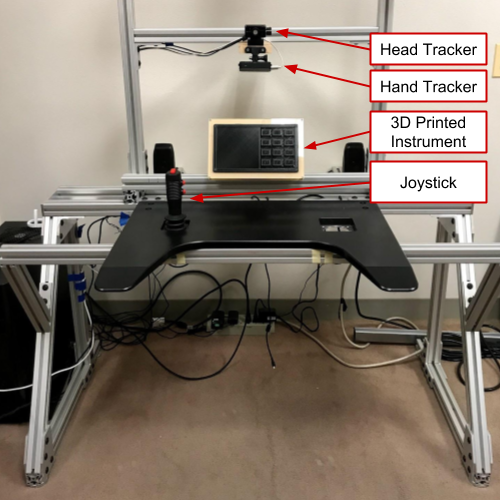
\includegraphics[width=\linewidth]{de_vr_photo.png}
        \caption{R3C Setup.}
        \label{fig:proto_design_exp:vr}
    \end{subfigure}
    \begin{subfigure}[t]{0.49\linewidth}
        \centering
        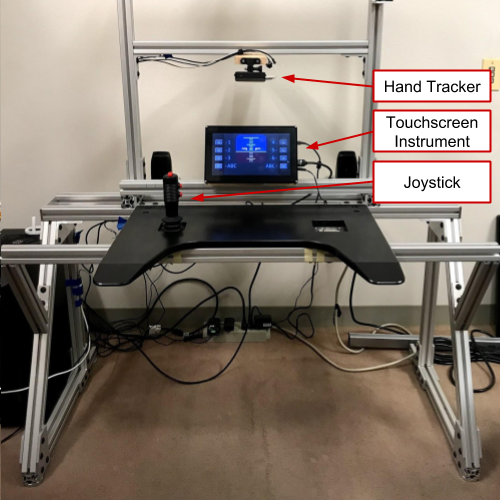
\includegraphics[width=\linewidth]{de_ts_photo.png}
        \caption{Touchscreen Setup.}
        \label{fig:proto_design_exp:ts}
    \end{subfigure}
    \caption{Simulator workstation for the third experiment.}
    \label{fig:proto_design_exp}
\end{figure}

With the improvements developed from the previous prototypes, the third prototype was designed to use only the hand tracker (without any capacitive touch sensors) to perform input on the 3D printed cockpit instrument buttons.
The hand tracker was mounted above the instrument and pointed towards the area in front of the instrument.
For a more realistic flight simulation, the task also involved using a joystick, which was mounted to the left of subjects at desk height.
To maintain realism, the joystick was modeled in the virtual environment, so that the movement of the joystick in the real world was visible to the subject in the virtual world.

\subsubsection{Calibration}

The virtual/real position registration calibration logic was modified for this setup to calibrate based off the position of the touchscreen.
This provided a very accurate and easy way to calibrate the hand tracker.
Instead of using the buttons on the instrument, requiring capacitive touch sensors on the buttons, the calibration was performed by switching to the touchscreen and pressing points on the screen.

We experienced some initial trouble with the calibration using a touchscreen due to the calibration points being contained in a single plane.
The problem this introduces is that the calibration least squares solution becomes over-fit to the plane, and causes any movement perpendicular to be scaled down near to the plane, causing the hand to appear to be `stuck' to the calibration plane.
To solve this, an artificial point was added at 1 inch outward from the middle of the sensor datum.
The same point was added as a known and measured point, forcing the calibration matrix to fit the entire tracking volume instead of just the plane.
This technique came from previous observations which showed that the accuracy of the sensor was improved as the hand neared the tracker.
After solving this issue, the calibration became very accurate with the touchscreen as the data source for known positions.

\section{Summary}

An overview of the technical approach of the evolving Rapidly Reconfigurable Research Cockpit was presented.
The final prototype achieved many of the goals set out by the motivations and requirements.
Developments that were outside the scope of this research work and could be undertaken as future work are discussed in Chapter~\ref{chap:conclusion}.
The specific configurations used in each experiment are described in detail within their respective chapter.
Some of the experiments required additional technology development that was not described here as the focus was on the R3C prototype itself.
